%
% Vorlage
%
% Stefan Taber <stefan.taber@inso.tuwien.ac.at>
%
\documentclass[a4paper,10pt,ngerman]{INSOexpose}
\inputencoding{utf8} % linux, mac
% \inputencoding{latin1} % linux, mac

%
%TODO Diese Informationen sind anzupassen
%
\title{
	\langchooser{
		Preliminary thesis title
	}{
		Durchführung einer Relay-Attacke durch Interception der Android NFC-Schnittstelle
	}
}
% Bitte setzen falls der Titel zu lang ist
%\shorttitle{Kurztitel}
\author{Michael Peyerl}
\matrikelnr{1326027}
\kennzahl{033 534}
\studium{Software \& Information Engineering}
\date{25.01.2018}
\dokumenttyp{%
	\langchooser{Bachelor Thesis}{Bachelorarbeit}
}
\assistent{}

% Bibliographie file
\bibliography{db}

\begin{document}
\maketitle

%=======================================================================
\section{\langchooser{Problem Description}{Problemstellung}}
%=======================================================================

\langchooser{
	General problem: Description of the concrete problem in a few sentences. Which topic is assigned to the job?
}{	
	Seit der Einigung auf die Entwicklung von Near-Field-Communication (NFC) durch Sony und Philips im Jahr 2002 \cite{sonyPhillipsNfcPressRelease} hat sich die Technologie stark weiterentwickelt. Das NFC Forum \cite{nfcForum} entwickelte zahlreiche Spezifikationen und die Frage nach Sicherheitsrisiken und -maßnahmen des neuen Kommunikationsmittels wurde vielfach behandelt \cite{nfcDevicesSecurityPrivacy, nfcTechVulnAttack, practExpNfcSecurity, nfcSecurityAnalysisAndVulnerabilities, securityNfc, nfcVulnerabilitiesDefense}. Im Jahr 2018 findet die NFC-Technologie Anwendung in zahlreichen unterschiedlichen Gebieten, von Autorisierung und Authentifizierung über mobile Haustürschlüssel bis zu bargeldlosem Bezahlen. Letztere ist höchstwahrscheinlich die bekannteste und am weitesten verbreitete Anwendung der relativ jungen Entwicklung. In nahezu jeder Debit- \footnote{http://www.kreditkarten.info/faq/was-ist-eine-debitkarte/} oder Kreditkarte ist bereits ein NFC-Chip integriert, über welchen an Point-of-Sales (POS) - Terminalen bargeldlos bezahlt werden kann. Zusätzlich verfügt ebenfalls der Großteil der heutzutage benutzten Smartphones über eine NFC-Schnittstelle, welche von Anwendungen benutzt werden kann, um mit einer auf dem mobilen Gerät gespeicherten Debit- oder Kreditkarte zu bezahlen. Mit steigender Prominenz kontaktloser Zahlungen über NFC, wird die Frage nach den Sicherheitsrisiken der Bezahlmethode immer relevanter. Ein Risiko, welches bereits vielfach erforscht wurde, welches allerdings nicht vollständig verhindert werden kann, ist die sogenannte Relay-Attacke \cite{nfcRelayWithOffTheShelfHardAndSoftware, pickingVirtualPockets, practicalNfcPeerToPeerRelayMobilePhones, practicalRelayContactlessTransactions, relayAttackOfNfcSmartCards, practicalNfcAttackmobileDevices, practicalExperiencesNfcRelayAndroid}. Bei diesem Angriff werden die NFC-Signale, die von einem POS-Terminal ausgehen, unverändert über einen zweiten Kommunikationskanal an ein weiteres Gerät (meistens werden hierfür Smartphones benutzt) gesendet. Dieses zweite Gerät befindet sich in unmittelbarer Nähe des Opfers und sendet diesem die empfangenen Signale über NFC. Die vom Opfer generierten Antworten werden wiederum unverändert an das erste Gerät gesendet, welches die Antwortsignale an das Terminal zurückgibt \cite{nfcTechVulnAttack}. Auf diese Art und Weise kann die kurze Distanz von NFC-Kommunikation überbrückt werden und so beispielsweise mit fremden Karten bezahlt werden, ohne dass diese sich in der Nähe des Terminals befinden. Die Durchführbarkeit dieser Attacke wurde bereits vielfach bewiesen und auch Gegenmaßnahmen wurden in der Literatur diskutiert. Es ergibt sich allerdings die noch nicht behandelte Fragestellung, ob es möglich ist, das Gerät des Opfers selbst (die NFC-Schnittstelle) so zu modifizieren, dass die NFC-Antwortsignale selbständig an ein weiteres mobiles Gerät gesendet werden, welches sich in der Nähe eines Terminals befindet. Sollte diese Angriffsmethode erfolgreich durchgeführt werden können, stellt sich in weiterer Folge die Frage nach Gegenmaßnahmen, um diese spezielle Ausführung einer Relay-Attacke zu verhindern. 
}
%=======================================================================
\section{\langchooser{Expected Results}{Zielsetzung/Motivation}}
%=======================================================================

\langchooser
{
	What is to be achieved through the thesis, what motivates you to this work?
}
{
	Durch diese Arbeit soll untersucht werden, ob bzw. wie es möglich ist, die Kommunikation einer Zahlungsanwendung mit der NFC-Schnittstelle so zu manipulieren, dass, nachdem NFC-Signale empfangen wurden, die Antworten über eine zweite Verbindung an ein anderes Gerät gesendet werden. Dieses befindet sich in der Nähe eines POS - Terminals und leitet die empfangenen Signale weiter. Dies ist eine spezielle Art einer Relay-Attacke, bei der allerdings im Gegensatz zu den meisten anderen Anwendungen dieser Angriffsweise nur ein Angreifer-Gerät erforderlich ist. Es wird außerdem davon ausgegangen, dass Root-Rechte auf dem Opfer-Gerät genutzt werden können, um die beschriebene Modifikation durchzuführen. 
	Darüber hinaus soll die Round-Trip-Time der NFC-Signale gemessen werden. Das ist "die Zeitspanne, die erforderlich ist, um ein Signal von einer Quelle über das Netzwerk zum Empfänger zu senden und die Antwort des Empfängers wiederum über das Netzwerk zurück zum Sender zu transportieren." \cite{rtt}. Das Signal, das über das Netzwerk gesendet wird (die sekundäre Verbindung) ist in diesem Fall die Application Protocol Data Unit (APDU) \footnote{https://de.wikipedia.org/wiki/Application\_Protocol\_Data\_Unit}.
	Ein Ziel der Arbeit ist daher die erfolgreiche Durchführung dieser speziellen Relay-Attacke bzw. die Modifikation des Opfer-Gerätes. Als weiteres Ziel sollen basierend auf Zeitmessungen der Signale Gegenmaßnahmen gefunden werden bzw. evaluiert werden, ob diese Attacke verhindert werden kann und wie eine Verhinderung möglich ist. 
	Darüber hinaus kann durch die Ergebnisse dieser Arbeit ein Grundstein gelegt werden um in weiterer Forschung zu untersuchen, ob die vorgestellte Modifikation des Opfer-Gerätes für weitere Angriffe oder Malware verwendet werden kann. Die Ergebnisse sollen in erster Linie dazu dienen, schädliche Nutzung zu unterbinden. 
}

%=======================================================================
\section{\langchooser{Methodological Approach}{Methodik}}
%=======================================================================

\langchooser
{
	Are there theoretical, pratical or empirical analyzes? Clear display of used theoretical and practical methods (survey, research, statistics, rapid prototyping, object oriented analysis, UML, component-based development, programming, etc.).
}
{
	In einem ersten Schritt wird ein Prototyp einer Android Mobile Payment Applikation mithilfe von Host-based Card Emulation (HCE)\footnote{https://developer.android.com/guide/topics/connectivity/nfc/hce.html} entwickelt. Dieser soll keine vollständige Zahlungs-Funktionalität zur Verfügung stellen, sondern in erster Linie in der Lage sein, mit einem POS-Terminal über die NFC-Schnittstelle des Smartphones zu kommunizieren. Das POS-Terminal wird durch einen Terminal Simulator\footnote{https://www.terminalsimulator.com/} auf einem Windows PC emuliert. Eine weitere Android-Applikation soll für die Kommunikation zwischen dem Opfer- und dem Angreifer-Gerät sorgen, wobei als sekundärer Kommunikationskanal eine drahtlose Verbindung über Bluetooth, WLAN oder das mobile Internet denkbar ist. Diese Kommunikations-Anwendung soll darüber hinaus auf dem Opfer-Gerät die HCE-App aktivieren. 
	Das Relay-Attack-Szenario ist in Abbildung 1 zur Veranschaulichung dargestellt.
	\newline
	\begin{figure}[h]
		\centering
		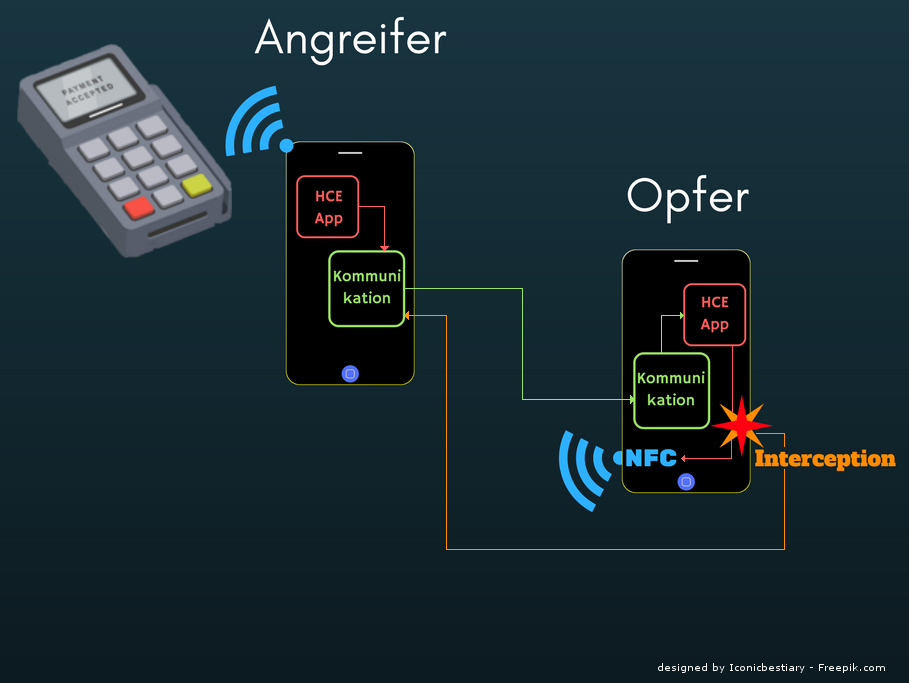
\includegraphics[width=10cm]{relay-szenario.png}
		\caption{Relay-Attack-Szenario}
	\end{figure} 
	\newline Diese Anwendungen sollen nativ mithilfe der Programmiersprachen Java und/oder Kotlin entwickelt werden. Nach erfolgreicher Implementierung soll recherchiert werden, auf welche Art und Weise die Kommunikation zwischen Android-App und der NFC-Schnittstelle des Smartphones auf das Angreifer-Gerät umgeleitet werden kann, um mithilfe der generierten Antwort-Signale auf dem POS-Terminal zahlen zu können. Hierfür wird es möglicherweise notwendig sein, mit dem Android-Framework direkt zu arbeiten bzw. ein System-Service (möglicherweise in C++) zu entwickeln. Schlussendlich soll die beschriebene Relay-Attacke erfolgreich durchgeführt werden. 
	Wurden diese Schritte abgeschlossen, wird evaluiert, wie ein derartiger Angriff verhindert werden kann. Um das zu erreichen, werden die Zeiten gemessen, die die NFC-Signale vom Opfer zum Angreifer und zurück benötigen. Basierend auf diesen Messungen kann festgestellt werden, ob es sinnvoll ist, zeitbasierte Protokolle zu entwickeln, welche diese Art von Angriff verhindern können. Falls der Rahmen der Arbeit dadurch nicht gesprengt wird, können weitere Gegenmaßnahmen getestet werden. 
}

%=======================================================================
\section{State of the Art}
%=======================================================================

\langchooser
{
	Existing solutions or similar projects of the topic. At least 5 references should be in this section.
}
{
	In zahlreichen Studien wurde bereits festgestellt, dass NFC Relay Attacken mit mobilen Geräten, die über eine NFC-Schnittstelle verfügen, einfach und ohne zusätzlichen Aufwand sowie ohne spezielles Fachwissen durchführbar sind und somit eine reelle und gefährliche Bedrohung für NFC-getriebene Services wie vor allem für mobile Zahlungen darstellen. 
	Im Jahr 2005 zeigten Ziv Kfir und Avishai Wool in einer der ersten Arbeiten über Relay Attacken \cite{practicalExperiencesNfcRelayAndroid} "Picking Virtual Pockets using Relay Attacks on Contactless Smartcard Systems" \cite{pickingVirtualPockets}, wie es mithilfe selbstgebauter Geräte möglich ist, das Signal einer Smartcard über eine Entfernung von 50 Meter an den NFC-Reader zu senden. Darüber hinaus wird auch beschrieben, wie die Distanz der Smartcard zum Proxy-Gerät auf bis zu 50 cm (um einen Faktor 5) erhöht werden kann. Zur Entstehung dieser Arbeit war für die Durchführung einer Relay-Attacke noch zusätzliche Hardware sowie elektrotechnisches Wissen notwendig.
	\newline
	Ohne zusätzliche Hardware können die Autoren der Arbeit "Practical NFC Peer-to-Peer Relay Attack Using Mobile Phones" \cite{practicalNfcPeerToPeerRelayMobilePhones} 5 Jahre später zeigen, wie mithilfe von zwei NFC-fähigen Mobiltelefonen die Peer-to-Peer Verbindung zweier weiterer NFC-fähiger Mobilgeräte durch eine Relay-Attacke weitergeleitet werden kann. Die NFC-Verbindung wird dabei über MIDlets \footnote{https://de.wikipedia.org/wiki/MIDlet} realisiert. Darüber hinaus wird in dieser Arbeit diskutiert, wie Relay-Attacken verhindert werden können, wobei Gegenmaßnahmen, die auf dem Standort der Geräte basieren, näher betrachtet werden. 
	\newline
	In Ihrem Artikel "Practical Relay Attack on Contactless Transactions by Using NFC Mobile Phones" \cite{practicalRelayContactlessTransactions} zeigen Lishoy Francis et al. ein Jahr später, wie mithilfe selbstentwickelter MIDlet-Applikationen eine Relay-Attacke über zwei handelsübliche Mobiltelefone durchgeführt werden kann. Nachdem ein mobiles Gerät als Proxy-Reader sowie das andere als Proxy-Token konfiguriert wurden, war es möglich die NFC-Signale in einem Test-Zahlungssystem sowie von einem e-Reisepass erfolgreich weiterzuleiten und in beiden Fällen wurden die Daten vom NFC-Reader akzeptiert. 
	\newline
	Mit fortschreitender Entwicklung wurden Relay-Attacken zunehmend einfacher. Xiquing Chu beschreibt in seiner Masterarbeit \cite{relayAttackOfNfcSmartCards} eine Relay-Attacke, die mit zwei Android Geräten durchgeführt wird, wobei keine zusätzliche Hardware und kaum zusätzliche Software benötigt wird. Zur Entstehung dieser Arbeit war die Android Version 4.4, welche Host Card Emulation einführt, soeben neu erschienen, weshalb der Autor noch eine ältere Android Version mit Cyanogenmod 9 verwendet. Zusätzlich wird die Zeit gemessen, die die einzelnen Kommandos benötigen und dabei wird festgestellt, dass die Relay-Attacke innerhalb der Frame Waiting Time (die maximale Antwortzeit nach Ende der Daten des Readers) \cite{practicalNfcAttackmobileDevices} durchgeführt werden kann. Abgesehen davon kann die Frame Waiting Time von Angreifern manipuliert werden und ist somit nicht für die Verhinderung einer Relay-Attacke geeignet \cite{practicalNfcAttackmobileDevices}.
	\newline
	Darüber hinaus beschreiben D. Cavdar et al. in ihrer Arbeit "A practical NFC relay attack on mobile devices using card emulation mode" \cite{practicalNfcAttackmobileDevices}, wie ein handelsübliches Smartphone ohne Hard- oder Software-Änderungen nur mithilfe einer selbstentwickelten App, die Host Card Emulation benutzt, verwendet werden kann, um Daten über NFC von einem anderen Gerät zu stehlen und diese bei einem NFC-Reader wiederzuverwenden, um sich unautorisierten Zugriff zu einem System zu verschaffen. Bemerkenswert hierbei ist, dass für die erfolgreiche Durchführung der Attacke nur ein einzelnes Smartphone ausreicht.
	\newline
	Eine ähnliche Arbeit liefern Jos\'{e} Vila et al. \cite{practicalExperiencesNfcRelayAndroid}, die eine Android-Applikation entwickelt haben, welche dem Gerät die Möglichkeit gibt, sowohl als NFC-Reader als auch als Smartcard zu operieren. Mithilfe dieser Anwendung gelang es den Autoren eine Relay-Attacke eines Zahlungssystems von New York nach Madrid über 5775 km durchzuführen. 
	\newline
	Thomas Bocek et al. \cite{nfcRelayWithOffTheShelfHardAndSoftware} führen ähnlich wie bereits zuvor beschrieben mithilfe zweier Android-Geräte, auf welchen Cyanogenmod installiert wurde, eine Relay-Attacke an öffentlichen POS-Terminals durch. Zusätzlich werden Gegenmaßnahmen wie Time Measurement und Distance Bounding diskutiert. 
}

%=======================================================================
\section{\langchooser{Table of Contents}{Inhaltsverzeichnis}}
%=======================================================================


\begin{samepage}
  \begin{contentstructure}
    \item Einleitung	\estimatedpages{3 Seiten}
	    \begin{contentstructure}
    	\item Problemstellung und Kontext der Arbeit
    	\item Ziel der Arbeit
    	\item Gliederung der Arbeit
    	\item Abgrenzung
	    \end{contentstructure}
    
    \item Grundlagen und Hintergründe \estimatedpages{10 - 13 Seiten}
	    \begin{contentstructure}
	    \item NFC
		    \begin{contentstructure}
	    	\item Technische Grundlagen
	    	\item Zahlungen mittels NFC
		   	\end{contentstructure}
	    \item NFC auf Android Geräten
		    \begin{contentstructure}
	    	\item Funktionsweise und Anwendung (NFC Schnittstelle)
	    	\item Host-based Card Emulation
		    \end{contentstructure}
	    \item NFC Sicherheitsrisiken und Angriffe
	    \item Relay Attacke
		    \begin{contentstructure}
	    	\item Prinzip
	    	\item Praktische Anwendung und Implementierung
	    	\item Gegenmaßnahmen
		    \end{contentstructure}
	    \item NFC Sicherheitsmaßnahmen
	    \end{contentstructure}
	\item Related Work \estimatedpages{2 Seiten}
    \item Implementierung der eigenen Relay-Attacke \estimatedpages{10 - 15 Seiten}
	    \begin{contentstructure}
	    \item Prinzip der Attacke
		\item Implementierung der HCE-Applikation
		\item Implementierung der Applikation für den sekundären Kommunikationskanal
		\item Interception der Kommunikation zwischen App und NFC-Schnittstelle
		\end{contentstructure}
	\item Analyse der Attacke \estimatedpages{7 - 10 Seiten}
		\begin{contentstructure}
		\item Resultate
			\begin{contentstructure}
			\item Zeitmessungen der NFC-Signale
			\item (Möglicherweise) Optimierung der Zeit
			\end{contentstructure}
		\item Anwendbarkeit
		\item Folgen und Risiken
		\end{contentstructure}
	\item Gegenmaßnahmen \estimatedpages{5 Seiten}
	\item Zusammenfassung \estimatedpages{1 Seite}
  \end{contentstructure}
\end{samepage}

%=======================================================================
%\section{Zeitplan}
%=======================================================================
% Zeitplanung der geplanten Arbeit mit wichtigen Meilensteine.

% Bibliographie
\printbibliography

\end{document}
